\documentclass[letterpaper,12pt]{article}

% Packages for better formatting
\usepackage{amsmath} 
\usepackage{graphicx} 
\usepackage{hyperref}
\usepackage{multirow}
\usepackage{colortbl}
\usepackage{listings}
\usepackage{minted}
\usepackage{xcolor}
\usepackage[T1]{fontenc}
\usepackage{indentfirst}
\usepackage{array}

%Code highlighting colors
\definecolor{commentblue}{rgb}{0.384, 0.447, 0.643}    % Pastel green for comments
\definecolor{numbercolor}{rgb}{0.722, 0.722, 0.722}   % Pastel gray for general code
\definecolor{codegreen}{rgb}{0.271, 0.459, 0.235}    % Pastel purple for strings
\definecolor{backcolour}{rgb}{0.969, 0.969, 0.9691}  % Very light gray for background
\definecolor{keycolour}{rgb}{0.8, 0.435, 0.361}

%Paragraph spacing options
\setlength{\parindent}{15pt}
\setlength{\parskip}{1em}

%Code listing style named "mystyle"
\lstdefinestyle{mystyle}{
  backgroundcolor=\color{backcolour},
  commentstyle=\color{commentblue},
  keywordstyle=\color{keycolour},
  numberstyle=\tiny\color{numbercolor},
  stringstyle=\color{codegreen},
  basicstyle=\ttfamily\footnotesize,
  breakatwhitespace=false,         
  breaklines=true,                 
  captionpos=b,                    
  keepspaces=true,                 
  numbers=left,                    
  numbersep=5pt,                  
  showspaces=false,                
  showstringspaces=false,
  showtabs=false,                  
  tabsize=2,
  frame=single,
  numbers=none,
  literate={"}{{\textquotedbl}}1
}

%"mystyle" code listing set
\lstset{style=mystyle}

% Title and author information
\title{\vspace{3cm}CSI4108: Cryptanalysis Project \vspace{2cm}}
\author{
    Danning Chen, 300234800
    \and
    Matthieu Ramanitrera, 300264295
}
\date{\vspace{2cm}\today}

\begin{document}

\maketitle

\newpage

\section{S-Box Design and Analysis}
Our randomly generated s-box is represented by the table below
    \begin{table}[ht]
        \centering
        \begin{tabular}{|c|c|c|c|c|c|c|c|c|c|c|c|c|c|c|c|}
            \hline
            0 & 1 & 2 & 3 & 4 & 5 & 6 & 7 & 8 & 9 & A & B & C & D & E & F \\
            \hline
            5 & 3 & A & 1 & E & D & 2 & 9 & 6 & F & C & 7 & B & 8 & 0 & 4 \\
            \hline
        \end{tabular}
        \caption{S-box Representation}
        \label{tab:sbox}
    \end{table}


For the permutation portion of the rounds we used the permutation given in Heys' tutorial \cite{heys}
\begin{table}[ht]
    \centering
    \begin{tabular}{|c|c|c|c|c|c|c|c|c|c|c|c|c|c|c|c|}
        \hline
        1 & 2 & 3 & 4 & 5 & 6 & 7 & 8 & 9 & 10 & 11 & 12 & 13 & 14 & 15 & 16 \\
        \hline
        1 & 5 & 9 & 13 & 2 & 6 & 10 & 14 & 3 & 7 & 11 & 15 & 4 & 8 & 12 & 16 \\
        \hline
    \end{tabular}
    \caption{Permutation}
    \label{tab:perm}
\end{table}

\subsection*{Initial analysis}
We build the difference distribution table, which was generated using Python (refer to Listing~\ref{lts:ddt} in the Appendix for the code). The difference distribution table is shown in Table~\ref{tab:ddt}.

\begin{table}[h]
    \centering
    \begin{tabular}{|cc|cccccccccccccccc|} 
    \cline{3-18}
    \multicolumn{1}{c}{~}                                                                                                                                                                                                                                   & ~          & \multicolumn{16}{c|}{\textbf{Output Difference}}                                                                                                                                                                                                                                                                                                                                                                                                                                                                                                                                                                                                                                                                                                                                                       \\
    \multicolumn{1}{c}{~}                                                                                                                                                                                                                                   & ~          & \textbf{0}                             & \textbf{1}                                     & \textbf{2}                                     & \textbf{3}                                     & \textbf{4}                                     & \textbf{5}                                     & \textbf{6}                                     & \textbf{7}                                     & \textbf{8}                                     & \textbf{9}                                     & \textbf{A}                                     & \textbf{B}                                     & \textbf{C}                                     & \textbf{D}                                     & \textbf{E}                                     & \textbf{F}                                      \\ 
    \hline
    \multirow{16}{*}{\begin{tabular}[c]{@{}c@{}}\textbf{I}\\\textbf{n}\\\textbf{p}\\\textbf{u}\\\textbf{t}\\\textbf{}\\\textbf{D}\\\textbf{i}\\\textbf{f}\\\textbf{f}\\\textbf{e}\\\textbf{r}\\\textbf{e}\\\textbf{n}\\\textbf{c}\\\textbf{e}\end{tabular}} & \textbf{0} & {\cellcolor[rgb]{0.902,0.902,0.902}}16 & {\cellcolor[rgb]{0.902,0.902,0.902}}0          & {\cellcolor[rgb]{0.902,0.902,0.902}}0          & {\cellcolor[rgb]{0.902,0.902,0.902}}0          & {\cellcolor[rgb]{0.902,0.902,0.902}}0          & {\cellcolor[rgb]{0.902,0.902,0.902}}0          & {\cellcolor[rgb]{0.902,0.902,0.902}}0          & {\cellcolor[rgb]{0.902,0.902,0.902}}0          & {\cellcolor[rgb]{0.902,0.902,0.902}}0          & {\cellcolor[rgb]{0.902,0.902,0.902}}0          & {\cellcolor[rgb]{0.902,0.902,0.902}}0          & {\cellcolor[rgb]{0.902,0.902,0.902}}0          & {\cellcolor[rgb]{0.902,0.902,0.902}}0          & {\cellcolor[rgb]{0.902,0.902,0.902}}0          & {\cellcolor[rgb]{0.902,0.902,0.902}}0          & {\cellcolor[rgb]{0.902,0.902,0.902}}0           \\
                                                                                                                                                                                                                                                            & \textbf{1} & 0                                      & 0                                              & 0                                              & \textbf{4}                                     & \textbf{2}                                     & 0                                              & \textbf{2}                                     & 0                                              & 0                                              & \textbf{2}                                     & 0                                              & \textbf{6}                                     & 0                                              & 0                                              & 0                                              & 0                                               \\
                                                                                                                                                                                                                                                            & \textbf{2} & {\cellcolor[rgb]{0.902,0.902,0.902}}0  & {\cellcolor[rgb]{0.902,0.902,0.902}}0          & {\cellcolor[rgb]{0.902,0.902,0.902}}\textbf{2} & {\cellcolor[rgb]{0.902,0.902,0.902}}0          & {\cellcolor[rgb]{0.902,0.902,0.902}}\textbf{2} & {\cellcolor[rgb]{0.902,0.902,0.902}}0          & {\cellcolor[rgb]{0.902,0.902,0.902}}0          & {\cellcolor[rgb]{0.902,0.902,0.902}}0          & {\cellcolor[rgb]{0.902,0.902,0.902}}\textbf{2} & {\cellcolor[rgb]{0.902,0.902,0.902}}0          & {\cellcolor[rgb]{0.902,0.902,0.902}}\textbf{2} & {\cellcolor[rgb]{0.902,0.902,0.902}}\textbf{2} & {\cellcolor[rgb]{0.902,0.902,0.902}}\textbf{4} & {\cellcolor[rgb]{0.902,0.902,0.902}}0          & {\cellcolor[rgb]{0.902,0.902,0.902}}0          & {\cellcolor[rgb]{0.902,0.902,0.902}}\textbf{2}  \\
                                                                                                                                                                                                                                                            & \textbf{3} & 0                                      & \textbf{2}                                     & 0                                              & \textbf{2}                                     & \textbf{2}                                     & 0                                              & 0                                              & \textbf{2}                                     & \textbf{2}                                     & \textbf{2}                                     & 0                                              & 0                                              & 0                                              & 0                                              & 0                                              & \textbf{4}                                      \\
                                                                                                                                                                                                                                                            & \textbf{4} & {\cellcolor[rgb]{0.902,0.902,0.902}}0  & {\cellcolor[rgb]{0.902,0.902,0.902}}0          & {\cellcolor[rgb]{0.902,0.902,0.902}}0          & {\cellcolor[rgb]{0.902,0.902,0.902}}\textbf{2} & {\cellcolor[rgb]{0.902,0.902,0.902}}0          & {\cellcolor[rgb]{0.902,0.902,0.902}}0          & {\cellcolor[rgb]{0.902,0.902,0.902}}0          & {\cellcolor[rgb]{0.902,0.902,0.902}}\textbf{2} & {\cellcolor[rgb]{0.902,0.902,0.902}}\textbf{4} & {\cellcolor[rgb]{0.902,0.902,0.902}}0          & {\cellcolor[rgb]{0.902,0.902,0.902}}0          & {\cellcolor[rgb]{0.902,0.902,0.902}}\textbf{2} & {\cellcolor[rgb]{0.902,0.902,0.902}}\textbf{2} & {\cellcolor[rgb]{0.902,0.902,0.902}}\textbf{2} & {\cellcolor[rgb]{0.902,0.902,0.902}}\textbf{2} & {\cellcolor[rgb]{0.902,0.902,0.902}}0           \\
                                                                                                                                                                                                                                                            & \textbf{5} & 0                                      & 0                                              & 0                                              & \textbf{4}                                     & \textbf{2}                                     & 0                                              & 0                                              & \textbf{2}                                     & \textbf{4}                                     & 0                                              & 0                                              & 0                                              & 0                                              & \textbf{2}                                     & \textbf{2}                                     & 0                                               \\
                                                                                                                                                                                                                                                            & \textbf{6} & {\cellcolor[rgb]{0.902,0.902,0.902}}0  & {\cellcolor[rgb]{0.902,0.902,0.902}}0          & {\cellcolor[rgb]{0.902,0.902,0.902}}0          & {\cellcolor[rgb]{0.902,0.902,0.902}}0          & {\cellcolor[rgb]{0.902,0.902,0.902}}\textbf{2} & {\cellcolor[rgb]{0.902,0.902,0.902}}0          & {\cellcolor[rgb]{0.902,0.902,0.902}}\textbf{2} & {\cellcolor[rgb]{0.902,0.902,0.902}}\textbf{4} & {\cellcolor[rgb]{0.902,0.902,0.902}}0          & {\cellcolor[rgb]{0.902,0.902,0.902}}0          & {\cellcolor[rgb]{0.902,0.902,0.902}}\textbf{2} & {\cellcolor[rgb]{0.902,0.902,0.902}}\textbf{2} & {\cellcolor[rgb]{0.902,0.902,0.902}}\textbf{2} & {\cellcolor[rgb]{0.902,0.902,0.902}}0          & {\cellcolor[rgb]{0.902,0.902,0.902}}0          & {\cellcolor[rgb]{0.902,0.902,0.902}}\textbf{2}  \\
                                                                                                                                                                                                                                                            & \textbf{7} & 0                                      & \textbf{2}                                     & \textbf{2}                                     & 0                                              & \textbf{2}                                     & 0                                              & 0                                              & \textbf{2}                                     & 0                                              & 0                                              & 0                                              & 0                                              & \textbf{4}                                     & 0                                              & 0                                              & \textbf{4}                                      \\
                                                                                                                                                                                                                                                            & \textbf{8} & {\cellcolor[rgb]{0.902,0.902,0.902}}0  & {\cellcolor[rgb]{0.902,0.902,0.902}}0          & {\cellcolor[rgb]{0.902,0.902,0.902}}\textbf{2} & {\cellcolor[rgb]{0.902,0.902,0.902}}\textbf{2} & {\cellcolor[rgb]{0.902,0.902,0.902}}0          & {\cellcolor[rgb]{0.902,0.902,0.902}}\textbf{4} & {\cellcolor[rgb]{0.902,0.902,0.902}}\textbf{4} & {\cellcolor[rgb]{0.902,0.902,0.902}}0          & {\cellcolor[rgb]{0.902,0.902,0.902}}0          & {\cellcolor[rgb]{0.902,0.902,0.902}}0          & {\cellcolor[rgb]{0.902,0.902,0.902}}0          & {\cellcolor[rgb]{0.902,0.902,0.902}}0          & {\cellcolor[rgb]{0.902,0.902,0.902}}\textbf{2} & {\cellcolor[rgb]{0.902,0.902,0.902}}\textbf{2} & {\cellcolor[rgb]{0.902,0.902,0.902}}0          & {\cellcolor[rgb]{0.902,0.902,0.902}}0           \\
                                                                                                                                                                                                                                                            & \textbf{9} & 0                                      & 0                                              & 0                                              & 0                                              & 0                                              & \textbf{2}                                     & \textbf{6}                                     & 0                                              & 0                                              & \textbf{2}                                     & \textbf{2}                                     & 0                                              & 0                                              & \textbf{4}                                     & 0                                              & 0                                               \\
                                                                                                                                                                                                                                                            & \textbf{A} & {\cellcolor[rgb]{0.902,0.902,0.902}}0  & {\cellcolor[rgb]{0.902,0.902,0.902}}\textbf{2} & {\cellcolor[rgb]{0.902,0.902,0.902}}0          & {\cellcolor[rgb]{0.902,0.902,0.902}}0          & {\cellcolor[rgb]{0.902,0.902,0.902}}\textbf{2} & {\cellcolor[rgb]{0.902,0.902,0.902}}0          & {\cellcolor[rgb]{0.902,0.902,0.902}}0          & {\cellcolor[rgb]{0.902,0.902,0.902}}0          & {\cellcolor[rgb]{0.902,0.902,0.902}}0          & {\cellcolor[rgb]{0.902,0.902,0.902}}\textbf{6} & {\cellcolor[rgb]{0.902,0.902,0.902}}0          & {\cellcolor[rgb]{0.902,0.902,0.902}}0          & {\cellcolor[rgb]{0.902,0.902,0.902}}\textbf{2} & {\cellcolor[rgb]{0.902,0.902,0.902}}0          & {\cellcolor[rgb]{0.902,0.902,0.902}}\textbf{4} & {\cellcolor[rgb]{0.902,0.902,0.902}}0           \\
                                                                                                                                                                                                                                                            & \textbf{B} & 0                                      & 0                                              & \textbf{4}                                     & 0                                              & 0                                              & \textbf{2}                                     & 0                                              & \textbf{2}                                     & 0                                              & 0                                              & \textbf{4}                                     & 0                                              & 0                                              & \textbf{2}                                     & 0                                              & \textbf{2}                                      \\
                                                                                                                                                                                                                                                            & \textbf{C} & {\cellcolor[rgb]{0.902,0.902,0.902}}0  & {\cellcolor[rgb]{0.902,0.902,0.902}}0          & {\cellcolor[rgb]{0.902,0.902,0.902}}\textbf{2} & {\cellcolor[rgb]{0.902,0.902,0.902}}0          & {\cellcolor[rgb]{0.902,0.902,0.902}}0          & {\cellcolor[rgb]{0.902,0.902,0.902}}\textbf{2} & {\cellcolor[rgb]{0.902,0.902,0.902}}0          & {\cellcolor[rgb]{0.902,0.902,0.902}}0          & {\cellcolor[rgb]{0.902,0.902,0.902}}\textbf{2} & {\cellcolor[rgb]{0.902,0.902,0.902}}0          & {\cellcolor[rgb]{0.902,0.902,0.902}}\textbf{2} & {\cellcolor[rgb]{0.902,0.902,0.902}}\textbf{2} & {\cellcolor[rgb]{0.902,0.902,0.902}}0          & {\cellcolor[rgb]{0.902,0.902,0.902}}0          & {\cellcolor[rgb]{0.902,0.902,0.902}}\textbf{6} & {\cellcolor[rgb]{0.902,0.902,0.902}}0           \\
                                                                                                                                                                                                                                                            & \textbf{D} & 0                                      & \textbf{4}                                     & 0                                              & 0                                              & 0                                              & \textbf{4}                                     & 0                                              & 0                                              & \textbf{2}                                     & 0                                              & 0                                              & \textbf{2}                                     & 0                                              & \textbf{2}                                     & \textbf{2}                                     & 0                                               \\
                                                                                                                                                                                                                                                            & \textbf{E} & {\cellcolor[rgb]{0.902,0.902,0.902}}0  & {\cellcolor[rgb]{0.902,0.902,0.902}}\textbf{2} & {\cellcolor[rgb]{0.902,0.902,0.902}}\textbf{2} & {\cellcolor[rgb]{0.902,0.902,0.902}}0          & {\cellcolor[rgb]{0.902,0.902,0.902}}\textbf{2} & {\cellcolor[rgb]{0.902,0.902,0.902}}\textbf{2} & {\cellcolor[rgb]{0.902,0.902,0.902}}\textbf{2} & {\cellcolor[rgb]{0.902,0.902,0.902}}\textbf{2} & {\cellcolor[rgb]{0.902,0.902,0.902}}0          & {\cellcolor[rgb]{0.902,0.902,0.902}}\textbf{2} & {\cellcolor[rgb]{0.902,0.902,0.902}}\textbf{2} & {\cellcolor[rgb]{0.902,0.902,0.902}}0          & {\cellcolor[rgb]{0.902,0.902,0.902}}0          & {\cellcolor[rgb]{0.902,0.902,0.902}}0          & {\cellcolor[rgb]{0.902,0.902,0.902}}0          & {\cellcolor[rgb]{0.902,0.902,0.902}}0           \\
                                                                                                                                                                                                                                                            & \textbf{F} & 0                                      & \textbf{4}                                     & \textbf{2}                                     & \textbf{2}                                     & 0                                              & 0                                              & 0                                              & 0                                              & 0                                              & \textbf{2}                                     & \textbf{2}                                     & 0                                              & 0                                              & \textbf{2}                                     & 0                                              & \textbf{2}                                      \\
    \hline
    \end{tabular}
    \caption{Difference Distribution Table}
    \label{tab:ddt}
    \end{table}


To find the best differential characteristic, we used the highest probabilities found in the differential distribution table while minimizing the number of active s-boxes at each round. We used the following difference pairs of the S-box:
\begin{align*}
    S_{12}&: \; \Delta X = D \rightarrow \Delta Y = 1 \; \text{with probability} \; \frac{4}{16} \\
    S_{24}&: \; \Delta X = 4 \rightarrow \Delta Y = 8 \; \text{with probability} \; \frac{4}{16} \\
    S_{31}&: \; \Delta X = 1 \rightarrow \Delta Y = 3 \; \text{with probability} \; \frac{4}{16}
\end{align*}

The input difference to the cipher is equivalent to the input difference to the first round (denoted $\Delta U_{1}$) which is:
\[
    \Delta P = \Delta U_{1} = [0000\;1101\;0000\;0000] = (0D00)_{16}
\]

The following is how this input difference propagates through the network for this specific differential characteristic where $\Delta U_{i}$
denotes the difference at the input of the i-th round S-boxes and $\Delta V_{i}$ the difference at the output of the i-th round S-boxes:\\

\begin{itemize}
    \item Round 1:  pick $ (\Delta X, \Delta Y) = (D, 1) \; \text{with probability} \; \frac{4}{16} $
    \begin{align*}
        \Delta U_{1} &=[0000\;1101\;0000\;0000] = (0D00)_{16} \\
        \Delta V_{1} &= [0000\;0001\;0000\;0000] = (0100)_{16}
    \end{align*}
    \[
        Probability = \frac{4}{16}
    \]

    \item Round 2:  pick $ (\Delta X, \Delta Y) = (4, 8) \; \text{with probability} \; \frac{4}{16} $
    \begin{align*}
        \Delta U_{2} &= [0000\;0000\;0000\;0100] = (0004)_{16} \\
        \Delta V_{2} &= [0000\;0000\;0000\;1000] = (0008)_{16}
    \end{align*}
    \[
        Probability = \frac{4}{16} \times \frac{4}{16}
    \]

    \item Round 3:  pick $ (\Delta X, \Delta Y) = (1, 3) \; \text{with probability} \; \frac{4}{16} $
    \begin{align*}
        \Delta U_{3} &= [0001\;0000\;0000\;0000] = (1000)_{16} \\
        \Delta V_{3} &= [0011\;0000\;0000\;0000] = (3000)_{16}
    \end{align*}
    \[
        Probability = \frac{4}{16} \times \frac{4}{16} \times \frac{4}{16}
    \]

    \item Input of Round 4 S-boxes: \\
    \begin{equation}
        \Delta U_{4} = [0000\;0000\;1000\;1000] = (0088)_{16}
    \end{equation}
    \[
        Probability = \frac{4}{16} \times \frac{4}{16} \times \frac{4}{16} = \frac{1}{64} = 0.015625 \label{eq:inputdiff}
    \]

\end{itemize}

Figure \ref{fig:dc} is a visual representation of the propagation of the input difference through the network.

\begin{figure}[h]
    \centering
    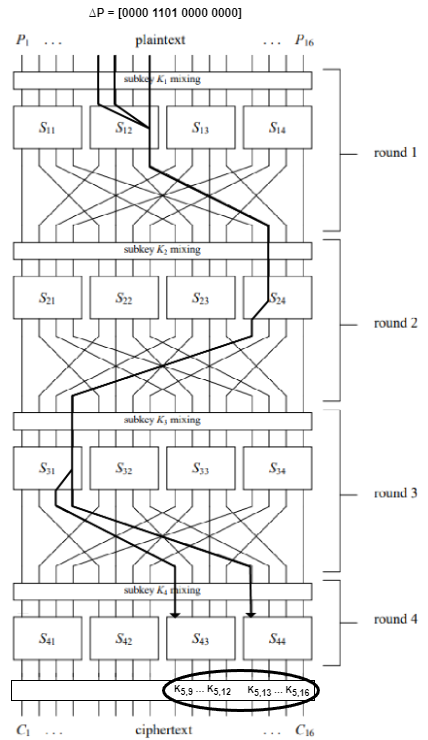
\includegraphics[width=0.8\textwidth]{sdc.png} % Change to your image filename
    \caption{Chosen Differential Characteristic}
    \label{fig:dc} % You can refer to this image by \ref{fig:sample-image}
\end{figure}

This differential characteristic has a probability of $ \frac{1}{16} \approx 0.0156$ to occur which is relatively high.
It allows us to try to guess the last two nibbles $ K_{5,9} ... K_{5,12} $ and $ K_{5,13} ... K_{5,16}$ of the fifth subkey used during the encryption process.

\clearpage

\section{Plaintext Generation and Encryption}
Since differential cryptanalysis is a chosen plaintext attack, we can generate plaintext pairs with the input difference
chosen in (\ref{eq:inputdiff}). Using Python, we each generated 5000 random 16-bit plaintexts and generated their respective plaintext pair by taking their exclusive-or 
with the desired input difference $ \Delta P = [0000\;1101\;0000\;0000] = (0D00)_{16} $. This gave us 10000 16-bit plaintext strings (5000 strings with their respective pair).

We then each ran the pairs through the Substitution-Permutation Network using a list of round keys not known by the other person and shared the output text files with each other to try to attack the cipher.
The details of the attacks are presented in Section~\ref{sec:attacks}.
The code for the implementation of the SPN can be found in the Appendix as Listing~\ref{lts:spn} as well as the code for plaintext pairs generation and encryption as Listing~\ref{lts:gen}.

\section{Differential attacks}
\label{sec:attacks}
\subsection{Person 1: Danning and Person 2: Matthieu}
The goal of the attack on this cipher was to try to guess bits of the last subkey used by Danning during the encryption of the plaintext pairs.
The differential characteristic presented above affects the inputs of S-boxes $S_{43}$ and $S_{44}$ so I could try to recover bits [$K_{5,9} \cdots K_{5,16}$]
from the fifth subkey.

First, I filtered the ciphertext pairs and only kept the ones for which the difference between them for the first 8 bits [$K_{5,1} \cdots K_{5,8}$] was zero.
That is because pairs having a non-zero difference in those bits couldn't be right pairs given the desired differential characteristic.

I then ran a partial decryption of the rest of the ciphertext string pairs up until the input of the 4-th round S-boxes.
I did so for all possible values of bits [$K_{5,9} \cdots K_{5,16}$] for the last subkey and incremented the count for that combination when the desired $\Delta U_{4} = (0088)_{16}$ occurred at the end.
Table~\ref{tab:resM} presents a portion of the data obtained from the subkey counts. The probability column indicate the estimated probability of occurence of right pairs for the candidate partial subkey as it was done in Heys' tutorial \cite{heys}.
The probability was calculated by dividing the count by the total number of ciphertext pairs (here 5000).

In this case, I was expecting the probability of occurrence of right pairs to be about $ p_{D} = 0.015625 $ and found out the highest probability among all candidates given by the partial subkey value [9,5] was $p_{D} = 0.0214$ which is noticeably higher.
It was revealed by Danning that this combination was indeed the one he used as the last byte of the final subkey so the attack was successful. The Python code for the subkey count and retrieval is given in Listing~\ref{lts:att} of the Appendix.

\begin{table}[h]
    \centering
    \begin{tabular}{|>{\centering\hspace{0pt}}m{0.338\linewidth}|>{\centering\hspace{0pt}}m{0.131\linewidth}|>{\centering\hspace{0pt}}m{0.338\linewidth}|>{\centering\arraybackslash\hspace{0pt}}m{0.131\linewidth}|} 
    \hline
    \textbf{Partial subkey} \par{}\textbf{[K\textsubscript{5,9} … K\textsubscript{5,16}]} & \textbf{Probability} & \textbf{Partial subkey} \par{}\textbf{[K\textsubscript{5,9} … K\textsubscript{5,16}]} & \textbf{Probability}  \\ 
    \hline
    8 C                                                                  & 0.0000               & 9 A                                                                  & 0.0000                \\
    \rowcolor[rgb]{0.902,0.902,0.902} 8 D                                & 0.0000               & 9 B                                                                  & 0.0000                \\
    8 E                                                                  & 0.0000               & 9 C                                                                  & 0.0000                \\
    \rowcolor[rgb]{0.902,0.902,0.902} 8 F                                & 0.0000               & 9 D                                                                  & 0.0000                \\
    9 0                                                                  & 0.0078               & 9 E                                                                  & 0.0020                \\
    \rowcolor[rgb]{0.902,0.902,0.902} 9 1                                & 0.0000               & 9 F                                                                  & 0.0000                \\
    9 2                                                                  & 0.0000               & A 0                                                                  & 0.0042                \\
    \rowcolor[rgb]{0.902,0.902,0.902} 9 3                                & 0.0098               & A 1                                                                  & 0.0000                \\
    9 4                                                                  & 0.0000               & A 2                                                                  & 0.0000                \\
    \rowcolor[rgb]{0.902,0.902,0.902} \textbf{9 5}                       & \textbf{0.0214}      & A 3                                                                  & 0.0042                \\
    9 6                                                                  & 0.0090               & A 4                                                                  & 0.0000                \\
    \rowcolor[rgb]{0.902,0.902,0.902} 9 7                                & 0.0052               & A 5                                                                  & 0.0076                \\
    9 8                                                                  & 0.0050               & A 6                                                                  & 0.0042                \\
    \rowcolor[rgb]{0.902,0.902,0.902} 9 9                                & 0.0022               & A 7                                                                  & 0.0022                \\
    \hline
    \end{tabular}
    \caption{Experimental Results for Differential Attack}
    \label{tab:resM}
    \end{table}

\subsection{Person 1: Matthieu and Person 2: Danning}
The attack is peformed in this process:
\begin{itemize}
    \item Generate the guessed key
    \item Loop through all cipher pairs
    \item Key mix with the ciphertext pair, then you get the guessed ciphertext pair before 5th key mixing
    \item S-box substitution with the inverse s box, then you get the cipher pair before 4th substitution.
    \item Compare the difference of the cipher pair with the expected difference, increase the count of this guessed key if they are the same.
    \item Increase the guessed key and go to step 2 again
\end{itemize}

The python code used to guess the last byte of the final subkey can be found in Listing~\ref{lts:attD} of the Appendix. When run on Matthieu's ciphertex pairs text file,
the program correcty guessed the last byte of the fifth subkey to be $(1E)_{16}$.

\newpage
\appendix
\section*{Appendix: Python Code}
\label{sec:appendix}

\subsection*{Generating the Difference Distribution Table}

Here is the Python code used to generate the difference distribution table:

\begin{lstlisting}[language=Python, caption=Python code for Difference Distribution Table (ddt.py), label=lts:ddt]
    import pandas as pd
    
    #S_Box
    s_box = [0x5, 0x3, 0xA, 0x1, 0xE, 0xD, 0x2, 0x9,
            0x6, 0xF, 0xC, 0x7, 0xB, 0x8, 0x0, 0x4]

    ddt = [[0 for _ in range(16)] for _ in range(16)]

    # Compute the DDT
    for x1 in range(16):
        for x2 in range(16):
            delta_x = x1 ^ x2
            delta_y = s_box[x1] ^ s_box[x2]
            ddt[delta_x][delta_y] += 1

    # Convert to DataFrame
    ddt_df = pd.DataFrame(ddt)
    print(ddt_df)
    \end{lstlisting}

\subsection*{Substitution-Permutation Network}

Here is a Python implementation of the Substitution-Permutation Network illustrated in Figure~\ref{fig:dc}:
    
\begin{lstlisting}[language=Python, caption=Python code for SPN (spn.py), label=lts:spn]
    def s_box(input):
        #Applies the s-box to a 4-bit input given as a 4 bit decimal integer.

        s_box_binary = [
            [0, 1, 0, 1],  # 0x5
            [0, 0, 1, 1],  # 0x3
            [1, 0, 1, 0],  # 0xA
            [0, 0, 0, 1],  # 0x1
            [1, 1, 1, 0],  # 0xE
            [1, 1, 0, 1],  # 0xD
            [0, 0, 1, 0],  # 0x2
            [1, 0, 0, 1],  # 0x9
            [0, 1, 1, 0],  # 0x6
            [1, 1, 1, 1],  # 0xF
            [1, 1, 0, 0],  # 0xC
            [0, 1, 1, 1],  # 0x7
            [1, 0, 1, 1],  # 0xB
            [1, 0, 0, 0],  # 0x8
            [0, 0, 0, 0],  # 0x0
            [0, 1, 0, 0]   # 0x4
        ]

        return s_box_binary[input]

    def permute(input):
        # Applies the permutation step to a 16-bit binary integer given as input.

        permutation_table = [0, 4, 8, 12, 1, 5, 9, 13, 2, 6, 10, 14, 3, 7, 11, 15]
        combined_input = [item for sublist in input for item in sublist]
        permuted = [0] * 16
        for i in range(16):
            permuted[permutation_table[i]] = combined_input[i]
        
        permuted_as_int = []
        for i in range(0, len(permuted), 4):
            permuted_as_int.append(binary_to_int(permuted[i:i+4]))
        
        return permuted_as_int

    def key_mix(input, round_key):
        # Mixes the round key to the input given as a list of 4 4-bit decimal integers

        divided_key = [(round_key >> 12) & 0xF,
                    (round_key >> 8) & 0xF,
                    (round_key >> 4) & 0xF,
                    round_key & 0xF]
        
        output = []
        for i in range(4):
            output.append(input[i] ^ divided_key[i])
        
        return output

    def spn(plaintext, round_keys):
        # Implements a 4-round SPN cipher

        current_input = process_plaintext(plaintext)
        for i in range(3):
            mixed = key_mix(current_input, round_keys[i])
            subbed = []
            for nibble in mixed:
                subbed.append(s_box(nibble))
            current_input = permute(subbed)
        
        final_sub = []
        for nibble in key_mix(current_input, round_keys[3]):
            final_sub.append(binary_to_int(s_box(nibble)))
        
        ciphertext = process_ciphertext(key_mix(final_sub, round_keys[4]))
        return ciphertext
        
            
    def binary_to_int(binary):
        # Helper function that converts a 4-bit binary integer to hexadecimal

        return int("".join(map(str, binary)), 2)

    def process_plaintext(plaintext):
        # Helper function to convert the 16-bit hexadecimal string into a list of 4 decimal integers

        nibbles = [(plaintext >> (4 * i)) & 0xF for i in range(4)]

        # The nibbles are in reverse order, so reverse them
        nibbles.reverse()
        return nibbles

    def process_ciphertext(ciphertext):
        # Helper function to convert a list of 4 decimal integers into a hexadecimal string

        hex_value = sum(nibble << (4 * i) for i, nibble in enumerate(reversed(ciphertext)))

        # Convert the integer to hexadecimal
        return hex(hex_value)
    \end{lstlisting}

\subsection*{Plaintext generation and encryption}
Here is the Python code used to generate and encrypt the plaintext pairs:

\begin{lstlisting}[language=Python, caption=Python code for plaintext pairs generation and encryption (generate.py), label=lts:gen]
    import random
    from spn import*

    def generate_pairs(input_difference, num_pairs=5000):
        ciphertext_pairs = []
        
        #Change the keys
        keys = [0x0000, 0x0000, 0x0000, 0x0000, 0x0000]

        for _ in range(num_pairs):
            # Generate a random plaintext
            plaintext1 = random.randint(0, 0xFFFF)
            # Calculate the second plaintext using the input difference
            plaintext2 = plaintext1 ^ input_difference
            
            # Encrypt both plaintexts
            ciphertext1 = spn(plaintext1, keys)
            ciphertext2 = spn(plaintext2, keys)

            # Store the plaintext pair and their corresponding ciphertexts
            ciphertext_pairs.append((ciphertext1, ciphertext2))

        return ciphertext_pairs

    def main():
        pairs = generate_pairs(0x0d00)

        # Output as a text file
        with open("ciphertext_pairs.txt", "w") as output_file:
            for pair in pairs:
                output_file.write(f"{pair[0]}, {pair[1]}\n")

    if __name__ == "__main__":
        main()
    \end{lstlisting}

\subsection*{Differential attack}
Here is the Python code used for the subkey count and retrieval of Danning's partial subkey:

\begin{lstlisting}[language=Python, caption=Python code for subkey count and retrieval by Matthieu, label=lts:att]
    import pandas as pd
    from spn import *
    def first_two_nibbles_equal(c1, c2):
        # Checks if two first nibbles (8 bits) of two strings are equal
        first_two_nibbles_1 = (c1 >> 8)
        first_two_nibbles_2 = (c2 >> 8)
        
        # Check if their values are equal
        return first_two_nibbles_1 == first_two_nibbles_2

    def reverse_sbox(input):
        # Reverse the S-box substitution
        rev_s_box = [14, 3, 6, 1, 15, 0, 8, 11, 13, 7, 2, 12, 10, 5, 4, 9]
        nibbles = [(input >> (4 * i)) & 0xF for i in range(4)]
        nibbles.reverse()
        output = 0
        for nibble in nibbles:
            output = (output << 4) | rev_s_box[nibble]
        
        return output
        
    def main():
        # Opening the ciphertext pairs file
        with open("ciphertext_pairs.txt") as f:
            pairs = []
            for line in f:
                values = line.strip().split(',')
                if len(values) == 2:
                    pair = (int(values[0].strip(), 16), int(values[1].strip(), 16))
                    pairs.append(pair)

        # Desired ciphertext difference in hex
        difference = 0x0088

        # Find pairs that have 0 difference in the first 8 bits
        possible_pairs = []
        for c1, c2 in pairs:
            if first_two_nibbles_equal(c1, c2):
                possible_pairs.append((c1, c2))
        
        key_count = [0] * 256
        for i in range(256):
            for c1, c2 in possible_pairs:
                # Reverse key mixing
                reversed_c1 = c1 ^ i
                reversed_c2 = c2 ^ i
                # Check difference at the entrance of the fourth round
                if reverse_sbox(reversed_c1) ^ reverse_sbox(reversed_c2) == difference:
                    key_count[i] += 1   # increment the count for that value
        
        probabilities = [count / 5000 for count in key_count]
        data = {
            'Partial subkey (hex)': [hex(i) for i in range(256)],
            'Probability': probabilities
        }
        df = pd.DataFrame(data)

        # Options to display the DataFrame
        pd.set_option('display.max_rows', None)
        pd.set_option('display.max_columns', None)
        pd.set_option('display.float_format', '{:.4f}'.format)
        # Display the DataFrame
        print(df.to_string(index=False))
        
        # The predicted value is the one with the highest count
        predicted_byte = hex(key_count.index(max(key_count)))
        print(f"Predicted byte for fifth round key: {predicted_byte}")

    if __name__ == "__main__":
        main()
    \end{lstlisting}

Here is Danning's Python code for the partial subkey retrieval:
    \begin{lstlisting}[language=Python, caption=Python code subkey retrieval by Danning, label=lts:attD]
    from collections import Counter

    TARGET_OUTPUT_DIFF = 0x0088

    def read_ciphertext_pairs(filename):

        ciphertext_pairs = []
        with open(filename, 'r') as file:
            for line in file:

                parts = line.strip().split(',')
            
                cipher_1 = f"{int(parts[0].strip(), 16):04x}"
                cipher_2 = f"{int(parts[1].strip(), 16):04x}"
    
                cipher_1_digits = [int(digit, 16) for digit in cipher_1]
                cipher_2_digits = [int(digit, 16) for digit in cipher_2]


                ciphertext_pairs.append((cipher_1_digits, cipher_2_digits ))

        return ciphertext_pairs

    def inverse_s_box(output):
        inverse_s_box_binary = [
        [1, 1, 1, 0],  # 0x0
        [0, 0, 1, 1],  # 0x1
        [0, 1, 1, 0],  # 0x2
        [0, 0, 0, 1],  # 0x3
        [1, 1, 1, 1],  # 0x4
        [0, 0, 0, 0],  # 0x5
        [1, 0, 0, 0],  # 0x6
        [1, 0, 1, 1],  # 0x7
        [1, 1, 0, 1],  # 0x8
        [0, 1, 1, 1],  # 0x9
        [0, 0, 1, 0],  # 0xA
        [1, 1, 0, 0],  # 0xB
        [1, 0, 1, 0],  # 0xC
        [0, 1, 0, 1],  # 0xD
        [0, 1, 0, 0],  # 0xE
        [1, 0, 0, 1]   # 0xF
    ]
        return inverse_s_box_binary[output]

    def process_plaintext(plaintext):

        nibbles = [(plaintext >> (4 * i)) & 0xF for i in range(4)]

        nibbles.reverse()
        return nibbles

    def binary_to_int(binary):
        return int("".join(map(str, binary)), 2)

    def partial_decrypt(input, subkey_guess):
    
        #key mixing with guessed subkey
        mixed = []
        for i in range(4):
            mixed.append(input[i] ^ subkey_guess[i])


        #undo the s_box substitution in round 4
        cipher_R4 = []
        for i in range(4):
            cipher_R4.append(binary_to_int(inverse_s_box(mixed[i])))
    
        return process_ciphertext(cipher_R4)

def process_ciphertext(ciphertext):
    hex_value = sum(nibble << (4 * i) for i, nibble in enumerate(reversed(ciphertext)))
    return hex(hex_value)

def generate_subkey_hex_digits(byte_value):

    assert 0 <= byte_value <= 0xFF, "Subkey byte must be between 0 and 255."
    high_nibble = (byte_value >> 4) & 0xF  
    low_nibble = byte_value & 0xF        
    subkey_hex_digits = [0, 0, high_nibble, low_nibble]
   
    return subkey_hex_digits

    def differential_attack(ciphertext_pairs, num_trials=1):

        #counter to track the frequency of each subkey guess
        subkey_guess_counts = Counter()

        for _ in range(num_trials):

            #loop through each ciphertext pair
            for cipher_1, cipher_2 in ciphertext_pairs:
                #possible values of the last byte of the 5th subkey
                for byte_value in range(0x00, 0x100):
                
                    #generate the subkey
                    subkey_guess_bits = generate_subkey_hex_digits(byte_value)

                    #partially decrypt cipher_1 and cipher_2 using the subkey guess
                    partial_decrypt_cipher_1 = partial_decrypt(cipher_1, subkey_guess_bits)
                    partial_decrypt_cipher_2 = partial_decrypt(cipher_2, subkey_guess_bits)


                
                    #check if the partial decryption result matches the target output difference
                    if (int(partial_decrypt_cipher_1, 16) ^ int(partial_decrypt_cipher_2, 16)) == TARGET_OUTPUT_DIFF:
                        subkey_guess_counts[byte_value] += 1


        fifth_subkey = subkey_guess_counts.most_common(1)[0][0]
        print(f"Last byte of the 5th subkey: {fifth_subkey :02X}")
        return


    ciphertext_pairs = read_ciphertext_pairs("ciphertext_pairs.txt")
    fifth_subkey  = differential_attack(ciphertext_pairs)
\end{lstlisting}

\begin{thebibliography}{99}
    \bibitem{heys} Howard M. Heys, A Tutorial on Linear and Differential Cryptanalysis
\end{thebibliography}

\end{document}
